% =====================================================================
%  MCMP117 -- Fundamentals of Operating Systems
%  Week 9 Course Notes: Linux Shell Basics & Filesystem Navigation
%  Compile with XeLaTeX (twice):  xelatex MCMP117_Week9_Notes.tex
%  Needs ./figures/ and the ../code/ folder.
% =====================================================================
\documentclass[11pt,a4paper]{article}
\newcommand{\weeknum}{9}
% ---------- Page & fonts ---------------------------------------------
\usepackage[a4paper,margin=2.3cm,headheight=15pt]{geometry}
\usepackage{fontspec}
\IfFontExistsTF{Calibri}{\setmainfont{Calibri}}{\setmainfont{Carlito}}
\IfFontExistsTF{Cambria}{\newfontfamily\headfont{Cambria}}{\newfontfamily\headfont{Caladea}}
\IfFontExistsTF{Consolas}{\setmonofont[Scale=0.95]{Consolas}}{\setmonofont[Scale=0.88]{DejaVu Sans Mono}}
\usepackage{amsmath,amssymb}
\usepackage{microtype}
\linespread{1.12}
\setlength{\parskip}{0.55em}
\setlength{\parindent}{0pt}

% ---------- Colours (course design system) ----------------------------
\usepackage{xcolor}
\definecolor{dark}{HTML}{212121}
\definecolor{charcoal}{HTML}{36454F}
\definecolor{slate}{HTML}{50808E}
\definecolor{mint}{HTML}{02C39A}
\definecolor{mintdeep}{HTML}{028090}
\definecolor{light}{HTML}{F2F2F2}
\definecolor{muted}{HTML}{6B7679}

% ---------- Packages ---------------------------------------------------
\usepackage{graphicx}
\usepackage{float}
\usepackage{needspace}
\graphicspath{{figures/}}
\usepackage[font=small,labelfont={bf,color=mintdeep},justification=centering]{caption}
\usepackage{booktabs,longtable,array,tabularx}
\usepackage{enumitem}
\setlist{itemsep=0.25em,topsep=0.3em}
\usepackage{tikz}
\usetikzlibrary{arrows.meta,positioning,calc,shapes.geometric}
\usepackage{pgfplots}
\pgfplotsset{compat=1.17}
\usepackage[most]{tcolorbox}
\usepackage{titlesec}
\usepackage{fancyhdr}
\usepackage{xurl}
\usepackage[colorlinks=true,linkcolor=mintdeep,urlcolor=mintdeep,citecolor=mintdeep]{hyperref}

% ---------- Headings ----------------------------------------------------
\titleformat{\section}{\headfont\Large\bfseries\color{charcoal}}{\color{mint}\thesection}{0.7em}{}
\titleformat{\subsection}{\headfont\large\bfseries\color{charcoal}}{\color{mintdeep}\thesubsection}{0.6em}{}
\titleformat{\subsubsection}{\headfont\normalsize\bfseries\color{mintdeep}}{}{0em}{}
\titlespacing*{\section}{0pt}{1.6em}{0.6em}
\titlespacing*{\subsection}{0pt}{1.2em}{0.4em}

% ---------- Header / footer -----------------------------------------------
\pagestyle{fancy}
\fancyhf{}
\fancyhead[L]{\small\color{muted}MCMP117 --- Fundamentals of Operating Systems}
\fancyhead[R]{\small\color{muted}Week \weeknum{} Notes}
\fancyfoot[C]{\small\color{muted}\thepage}
\renewcommand{\headrulewidth}{0pt}

% ---------- Boxes ---------------------------------------------------------
\newtcolorbox{keyidea}[1][Key idea]{enhanced,breakable,colback=charcoal,colframe=charcoal,
  coltext=white,fonttitle=\headfont\bfseries\color{mint},title={#1},
  attach title to upper={\par\smallskip},boxrule=0pt,arc=3pt,left=10pt,right=10pt,top=8pt,bottom=8pt}
\newtcolorbox{example}[1][Worked example]{enhanced,colback=light,colframe=light,
  fonttitle=\headfont\bfseries\color{mintdeep},title={#1},attach title to upper={\par\smallskip},
  boxrule=0pt,arc=3pt,left=10pt,right=10pt,top=8pt,bottom=8pt}
\newtcolorbox{tryit}[1][Try it yourself]{enhanced,breakable,colback=white,colframe=mint,
  fonttitle=\headfont\bfseries\color{mintdeep},title={#1},attach title to upper={\par\smallskip},
  boxrule=0.8pt,arc=3pt,left=10pt,right=10pt,top=8pt,bottom=8pt}
\newtcolorbox{histnote}[1][Historical note]{enhanced,breakable,colback=white,colframe=slate!40,
  fonttitle=\headfont\bfseries\color{slate},title={#1},attach title to upper={\par\smallskip},
  boxrule=0.5pt,arc=3pt,left=10pt,right=10pt,top=8pt,bottom=8pt,fontupper=\small}

% Photo helper: fits image inside a box, never distorted (keepaspectratio)
\newcommand{\photo}[3]{\includegraphics[width=#1,height=#2,keepaspectratio]{#3}}

\newcommand{\term}[1]{\textbf{\color{mintdeep}#1}}
\newcommand{\cmd}[1]{\texttt{#1}}


% ---------- Code listings ----------------------------------------------------
\usepackage{listings}
\lstdefinestyle{course}{
  basicstyle=\ttfamily\small, columns=fullflexible, keepspaces=true,
  backgroundcolor=\color{dark}, rulecolor=\color{dark}, frame=single, framesep=6pt,
  xleftmargin=8pt, xrightmargin=8pt, aboveskip=0.8em, belowskip=0.6em,
  basicstyle=\ttfamily\small\color{light},
  keywordstyle=\color{mint}\bfseries, commentstyle=\color{white!60}\itshape,
  stringstyle=\color{orange!70!yellow}, numberstyle=\tiny\color{muted},
  numbers=left, numbersep=10pt, showstringspaces=false, breaklines=true,
  tabsize=4, upquote=true}
\lstdefinestyle{term}{style=course, numbers=none, keywordstyle=\color{light},
  commentstyle=\color{white!60}, stringstyle=\color{light}}
\lstset{style=course,language=C}
\usepackage{textcomp}

\begin{document}
% ============================ Week 9 body ============================
% Terminal transcripts are read directly from ../code/out_*.txt (real captured output).
\newcommand{\outl}[3]{\Needspace{5\baselineskip}\lstinputlisting[style=term,firstline=#2,lastline=#3]{../code/#1}}
\newcommand{\tl}{\textasciitilde}
\lstdefinestyle{term}{style=course, numbers=none, keywordstyle=\color{light},
  commentstyle=\color{white!60}, stringstyle=\color{light}, basicstyle=\ttfamily\footnotesize\color{light}}
\sloppy

\thispagestyle{empty}
\begin{tcolorbox}[enhanced,colback=dark,colframe=dark,arc=0pt,boxrule=0pt,
  left=18pt,right=18pt,top=20pt,bottom=20pt,coltext=white]
{\small\color{mint}\textsc{MCMP117 \,·\, Week 9 \,·\, Course Notes}}\par\medskip
{\headfont\fontsize{26}{30}\selectfont\bfseries Fundamentals of Operating Systems}\par\medskip
{\large Linux Shell Basics \& Filesystem Navigation}\par\smallskip
{\small\itshape\color{white!70} From theory to the terminal: where am I, what is here, and how do I move?}
\end{tcolorbox}

\vspace{0.4em}
{\small
\textbf{Instructor:} Asst.\ Prof.\ Dr.\ (Ph.D.) Hasan Oğuz\\
Head of the Electronical Communication Technology Programme, Vocational School\\
Istanbul Okan University\par}

\vspace{0.8em}
\begin{keyidea}[What you should be able to do after this week]
\begin{enumerate}[leftmargin=1.4em]
  \item Open a Linux terminal on a lab PC, with WSL on Windows, or in a VirtualBox virtual machine, and create the course lab folder \texttt{\tl/lab}.
  \item Explain the difference between the terminal, the shell and the kernel, and describe what happens (fork, exec, wait, system calls) when you type a command.
  \item Read the prompt and split a command line into command, options and arguments.
  \item Use \cmd{whoami}, \cmd{hostname}, \cmd{date}, \cmd{echo}, \cmd{uname}, \cmd{pwd} and \cmd{ls} with its most useful options, and read every column of \cmd{ls -l}.
  \item Describe the Linux directory tree (\texttt{/}, \texttt{/home}, \texttt{/etc}, \texttt{/bin}, \texttt{/usr}, \texttt{/var}, \texttt{/tmp}, \texttt{/dev}, \texttt{/proc}).
  \item Move around with \cmd{cd} using absolute and relative paths and the special names \texttt{\tl}\ \texttt{.}\ \texttt{..}\ \texttt{-}; explain why \cmd{cd} is a shell builtin.
  \item Find help (\cmd{--help}, \cmd{man}, \cmd{help}, \cmd{type}) and work efficiently with tab completion, history and keyboard shortcuts.
\end{enumerate}
\end{keyidea}

\setcounter{tocdepth}{1}
\tableofcontents

% =====================================================================
\section{From the Midterm to the Terminal}

The first half of the course (Weeks~1--7, examined in the Week~8 midterm) was about \emph{ideas}: the operating system as resource manager and extended machine, the kernel running in kernel mode while everything else runs in user mode, \term{system calls} as the only door into the kernel (Weeks~2--3), \term{processes} with their PID, state and PCB, created with \cmd{fork()} and \cmd{exec()} and scheduled by the CPU scheduler (Weeks~3--5), and finally memory, virtual memory, files and the tree-structured directory (Weeks~6--7).

From this week until Week~14 we work \emph{hands-on} in the Linux shell. You will see the same ideas at work: every command you type becomes a process; every file listing is read from a directory through a system call; the directory tree of Week~7 is the tree you walk with \cmd{cd}. Week~10 covers file operations, Week~11 permissions, Week~12 text processing and pipes, Week~13 processes and job control, and Week~14 shell scripting.
\paragraph{About the outputs in these notes.} All terminal output was captured on Ubuntu 24.04 LTS with a normal user called \texttt{student} on a computer called \texttt{okan-lab}, with the locale \texttt{LC\_ALL=C.UTF-8}. On your machine the user name, host name, dates, times, sizes of system files and process IDs (PIDs) will be different, and with another locale the sort order of \cmd{ls} may differ slightly (for example, whether upper-case names come first). The files inside \texttt{\tl/lab} are identical for everybody. Ubuntu also colours the output of \cmd{ls} (directories in blue); our captured output has no colours. Every demo is in the \texttt{code/} folder as a \texttt{demo\_*.sh} file with its output in \texttt{out\_*.txt}.

% =====================================================================
\section{Getting a Linux Terminal}
\label{sec:getlinux}

You need a Linux shell for the rest of the semester. There are three good ways to get one; the commands are the same in all three.


\subsection{Option 1: the lab PCs}
Log in, open the \emph{Terminal} application and continue with Section~\ref{sec:labsetup}. \emph{[The exact room, account and system on the lab PCs will be announced by the instructor.]}

\subsection{Option 2: WSL on Windows 10/11}
The \term{Windows Subsystem for Linux} (WSL) runs a real Linux kernel in a lightweight virtual machine managed by Windows, with Ubuntu as the default distribution.

\begin{enumerate}[leftmargin=1.4em]
  \item Right-click the Start button and choose \emph{Terminal (Admin)} or \emph{Windows PowerShell (Admin)}.
  \item Type the following command and press Enter:
\begin{lstlisting}[style=term]
PS C:\Windows\system32> wsl --install
\end{lstlisting}
  It enables the necessary Windows features, installs WSL~2 and downloads Ubuntu.
  \item Restart Windows when asked.
  \item Open \emph{Ubuntu} from the Start menu. On the first start it asks for a new \emph{Linux} user name and password (they do not have to match your Windows account). While you type the password \emph{nothing is shown}, not even stars --- this is normal on Linux. This user may later run administrator commands with \cmd{sudo}.
  \item From now on open \emph{Ubuntu} (or type \cmd{wsl} in PowerShell) whenever you need the shell.
\end{enumerate}

Useful facts: \cmd{wsl -l -v} (in PowerShell) lists the installed distributions and their WSL version; \cmd{wsl --install -d Ubuntu-24.04} installs a particular Ubuntu release. Inside Linux, your Windows \texttt{C:} drive appears as \texttt{/mnt/c}, so your Windows downloads folder is \texttt{/mnt/c/Users/<your Windows name>/Downloads}. If installation fails with a message about virtualization, enable it in the BIOS/UEFI setup of your computer (it is called Intel VT-x, AMD-V or SVM).

\subsection{Option 3: VirtualBox and Ubuntu}
A \term{virtual machine} applies the OS idea of virtualization to a whole computer: a \emph{hypervisor} (here VirtualBox) gives the guest OS virtual CPUs, memory and a virtual disk, so Ubuntu runs as if it owned the hardware.

\begin{enumerate}[leftmargin=1.4em]
  \item Download and install VirtualBox, and download the \emph{Ubuntu Desktop 24.04 LTS} ISO image (about 6\,GB).
  \item In VirtualBox click \emph{New}: give the VM a name, select the ISO image, type Linux / Ubuntu (64-bit).
  \item Give it $4096$\,MB of memory, $2$ CPUs and a $25$\,GB virtual disk (dynamically allocated: the file grows only as needed). If your laptop has only 4\,GB of RAM, prefer WSL.
  \item Start the VM and follow \emph{Install Ubuntu}. The option ``Erase disk and install Ubuntu'' erases only the \emph{virtual} disk, a file on your computer --- not your Windows disk. (VirtualBox~7 can also do an ``unattended installation'' that fills in the user details for you.)
  \item Log in and open a terminal with \texttt{Ctrl+Alt+T} (or \emph{Activities} $\to$ \emph{Terminal}).
\end{enumerate}

\paragraph{Mac users.} The macOS Terminal (with the shell \cmd{zsh}) understands most commands of this week, but many options of the BSD tools on macOS differ from the GNU tools on Linux. For the coming weeks use a Linux VM (on Apple Silicon Macs, UTM is a free option; VirtualBox support there is limited).

\subsection{Creating the lab folder}
\label{sec:labsetup}

All practical weeks use the same practice folder \texttt{\tl/lab}. It is created by the script \texttt{mcmp117\_lab\_setup.sh}, which you find in the \texttt{code/} folder of every Linux week and in the course's GitHub repository. Run it \emph{once} with \cmd{bash}; it always builds the folder \texttt{lab} in your home directory, wherever the script itself is:

\begin{lstlisting}[style=term]
# Ubuntu / VM: the script is in your Downloads folder
student@okan-lab:~$ bash ~/Downloads/mcmp117_lab_setup.sh
# WSL: the script is in your Windows Downloads folder (use your Windows name)
student@okan-lab:~$ bash /mnt/c/Users/ayse/Downloads/mcmp117_lab_setup.sh
\end{lstlisting}

With the script in the home directory, the real output looks like this (\cmd{ls} lists a directory; Section~\ref{sec:ls}):
\outl{out_setup.txt}{1}{12}

The script contains no randomness: everybody gets exactly the same files as these notes. It is safe to run again --- it deletes and re-creates \emph{only} the folder \texttt{lab} --- so whenever your lab folder gets into a mess, simply run it again. For the same reason, never keep your own work inside \texttt{\tl/lab}.

\begin{tryit}[If the script fails]
If you see an error such as \texttt{line 2: \$'\textbackslash r': command not found}, the file got Windows line endings (for example after being opened and saved in Notepad). Download it again, or repair it with \cmd{sed -i 's/\textbackslash r\$//' mcmp117\_lab\_setup.sh}. If you see \texttt{No such file or directory}, check the path with \cmd{ls} first (Section~\ref{sec:errors}).
\end{tryit}

% =====================================================================
\section{Terminal, Shell and Kernel}

\subsection{Three programs, three jobs}

People often use ``terminal'', ``shell'', ``command line'' and ``Linux'' as if they meant the same thing. They are different layers:

\begin{figure}[H]
\centering
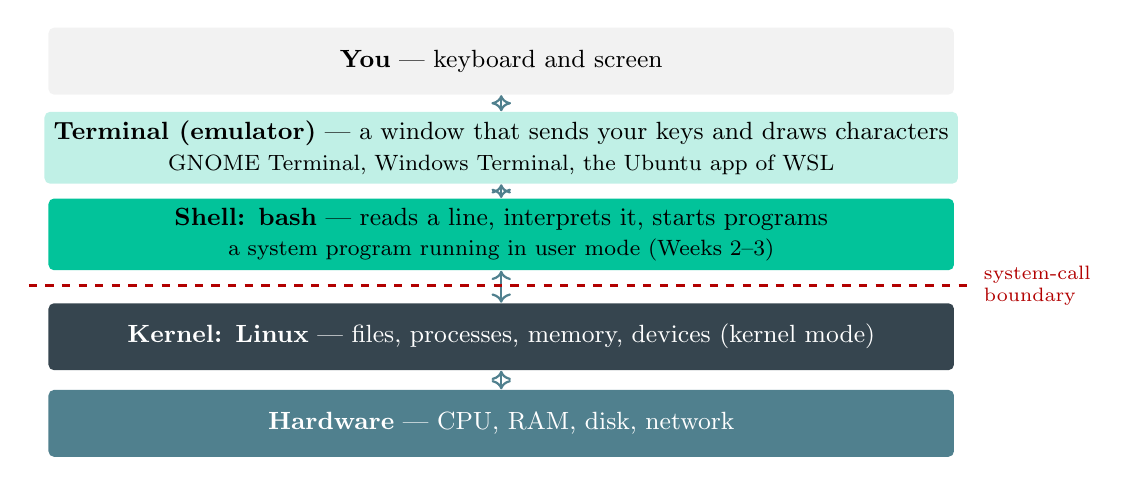
\begin{tikzpicture}[l/.style={rectangle,rounded corners=2pt,minimum width=11.5cm,minimum height=0.85cm,align=center,font=\small}]
\node[l,fill=light] (u) at (0,0) {\textbf{You} --- keyboard and screen};
\node[l,fill=mint!25] (t) at (0,-1.1) {\textbf{Terminal (emulator)} --- a window that sends your keys and draws characters\\{\footnotesize GNOME Terminal, Windows Terminal, the Ubuntu app of WSL}};
\node[l,fill=mint] (s) at (0,-2.2) {\textbf{Shell: bash} --- reads a line, interprets it, starts programs\\{\footnotesize a system program running in user mode (Weeks 2--3)}};
\node[l,fill=charcoal,text=white] (k) at (0,-3.5) {\textbf{Kernel: Linux} --- files, processes, memory, devices (kernel mode)};
\node[l,fill=slate,text=white] (h) at (0,-4.6) {\textbf{Hardware} --- CPU, RAM, disk, network};
\draw[<->,slate,thick] (u) -- (t); \draw[<->,slate,thick] (t) -- (s); \draw[<->,slate,thick] (k) -- (h);
\draw[<->,slate,thick] (s) -- (k);
\draw[dashed,red!70!black,thick] (-6,-2.85) -- (6,-2.85) node[right,font=\scriptsize,align=left] {system-call\\boundary};
\end{tikzpicture}
\caption{The layers between you and the hardware. Everything above the dashed line runs in user mode.}
\end{figure}

\begin{itemize}
  \item The \term{terminal} only handles input and output. It does not understand commands. (Historically a terminal was a physical device --- a teletype or a video terminal such as the VT100; today it is a program that emulates one.)
  \item The \term{shell} is the \emph{command interpreter} of Week~3. Linux offers several: \cmd{bash} (the default on Ubuntu), \cmd{zsh}, \cmd{sh}, \cmd{fish}. As Week~2 stressed, the shell is \emph{not} part of the kernel; it is an ordinary system program.
  \item The \term{kernel} does the real work for every command, and is reached only through system calls.
  \item Strictly, ``Linux'' is only the kernel; Ubuntu is a \emph{distribution}: the Linux kernel plus the GNU tools (\cmd{bash}, \cmd{ls}, \ldots) and thousands of other programs.
\end{itemize}

\subsection{What happens when you type a command}
\label{sec:forkexec}

When you type \cmd{ls} and press Enter, \cmd{bash} works through the \emph{fork--exec--wait} pattern of Week~3:

\begin{figure}[H]
\centering
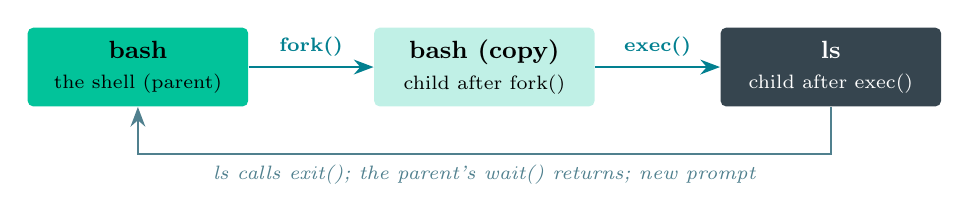
\begin{tikzpicture}[b/.style={rectangle,rounded corners=2pt,minimum width=2.8cm,minimum height=1.0cm,align=center,font=\small},
  arr/.style={-{Stealth[length=2.5mm]},thick,mintdeep}]
\node[b,fill=mint] (p) at (0,0) {\textbf{bash}\\{\scriptsize the shell (parent)}};
\node[b,fill=mint!25] (c) at (4.4,0) {\textbf{bash (copy)}\\{\scriptsize child after fork()}};
\node[b,fill=charcoal,text=white] (l) at (8.8,0) {\textbf{ls}\\{\scriptsize child after exec()}};
\draw[arr] (p) -- node[above,font=\scriptsize\bfseries]{fork()} (c);
\draw[arr] (c) -- node[above,font=\scriptsize\bfseries]{exec()} (l);
\draw[arr,slate] (l.south) -- ++(0,-0.6) -| node[pos=0.25,below,font=\scriptsize\itshape]{ls calls exit(); the parent's wait() returns; new prompt} (p.south);
\end{tikzpicture}
\caption{The shell creates a new process for every external command.}
\end{figure}

\begin{enumerate}[leftmargin=1.4em]
  \item \textbf{Read:} \cmd{bash} reads the line \texttt{ls} from the terminal.
  \item \textbf{Find:} \cmd{ls} is not a builtin, so \cmd{bash} searches the directories listed in the variable \texttt{\$PATH} and finds the program file \texttt{/usr/bin/ls}.
  \item \textbf{fork():} \cmd{bash} creates a child process, a copy of itself, with a new PID.
  \item \textbf{exec():} the child replaces its program with \texttt{/usr/bin/ls}, which runs, prints and exits.
  \item \textbf{wait():} the parent shell waits for the child to finish and then prints the next prompt.
\end{enumerate}

Some commands, called \term{builtins}, are executed by \cmd{bash} itself without creating a process: \cmd{cd}, \cmd{pwd}, \cmd{echo}, \cmd{history}, \cmd{type} and others. Section~\ref{sec:cdbuiltin} explains why \cmd{cd} \emph{has} to be a builtin.

\subsection{Commands become system calls}

In Week~2 we used \cmd{strace} to list the system calls of a C program. It works for any command. Here we trace only three kinds of system call, and \texttt{> /dev/null} throws away the normal output of \cmd{ls} so that only the report of \cmd{strace} remains (redirection is the topic of Week~12):

\outl{out_syscalls.txt}{2}{7}

\begin{itemize}
  \item \texttt{execve}: the child process becomes \texttt{/usr/bin/ls} with the argument list \texttt{["ls", "docs"]} --- step~4 above.
  \item \texttt{getdents64} (``get directory entries'') reads the directory. It found $9$ entries: the $6$ visible files, the hidden file \texttt{.settings}, and the two entries \texttt{.} and \texttt{..} that every directory contains. A second call returns $0$ entries: the end of the directory. Recall from Week~7 that a directory is a file containing (name, inode number) pairs; this is the system call that reads those pairs.
  \item \texttt{write(1, \ldots, 86)} writes $86$ bytes to file descriptor~$1$, standard output.
\end{itemize}
\cmd{ls} cannot read the disk on its own; like every user-mode program it must ask the kernel (dual mode, Week~2). Without the filter, \cmd{ls} makes several dozen system calls (loading libraries, reading locale files, mapping memory). If \cmd{strace} is missing: \cmd{sudo apt install strace}.

% =====================================================================
\section{The Prompt and Your First Commands}

\subsection{Reading the prompt}

When the shell is ready for a command it prints a \term{prompt}. The default Ubuntu prompt has the form \texttt{user@host:directory\$}:

\begin{center}
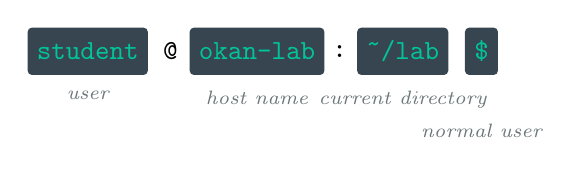
\begin{tikzpicture}[p/.style={rectangle,rounded corners=1.5pt,fill=charcoal,text=mint,font=\ttfamily,minimum height=0.6cm},
  q/.style={font=\ttfamily}, lab/.style={font=\scriptsize\itshape,text=muted}]
\node[p] (a) at (0,0) {student}; \node[q] at (1.05,0) {@};
\node[p] (b) at (2.15,0) {okan-lab}; \node[q] at (3.2,0) {:};
\node[p] (c) at (4.0,0) {\textasciitilde/lab}; \node[p] (d) at (5.0,0) {\$};
\node[lab,below=2pt of a] {user}; \node[lab,below=2pt of b] {host name};
\node[lab,below=2pt of c] {current directory}; \node[lab,below=14pt of d] {normal user};
\end{tikzpicture}
\end{center}

The tilde \texttt{\tl} is short for your \term{home directory}, here \texttt{/home/student}. A prompt ending in \texttt{\#} instead of \texttt{\$} means you are \texttt{root}, the administrator --- be careful then. In these notes, the text after the prompt is what you type; the lines without a prompt are the output.

\subsection{Anatomy of a command}

A command line is split at spaces into \emph{words}:
\begin{center}
\texttt{\textbf{command}\ \ -options\ \ arguments}\qquad e.g.\qquad \texttt{ls -l -a docs}
\end{center}
\begin{itemize}
  \item The first word is the \term{command}: a program file or a builtin.
  \item \term{Options} change \emph{how} the command works. Short options are one letter after a dash and can be combined: \cmd{ls -l -a} $=$ \cmd{ls -la} $=$ \cmd{ls -al}. Long options start with two dashes and are spelled out: \cmd{ls --all}. Some options take a value: \cmd{head -n 4}.
  \item \term{Arguments} say \emph{what} the command works on: files, directories, text.
\end{itemize}
Linux is \emph{case-sensitive}: \cmd{ls} and \cmd{LS} are different words, and so are \texttt{docs} and \texttt{Docs}. The spaces matter too: \cmd{ls-l} is one word, a command that does not exist.

\begin{center}
\begin{tabular}{l l l l}
\toprule
\textbf{Example} & \textbf{Command} & \textbf{Options} & \textbf{Arguments}\\
\midrule
\texttt{pwd} & \texttt{pwd} & --- & ---\\
\texttt{ls -la docs} & \texttt{ls} & \texttt{-l -a} (combined) & \texttt{docs}\\
\texttt{ls --all docs} & \texttt{ls} & \texttt{--all} (long form) & \texttt{docs}\\
\texttt{cd ../src} & \texttt{cd} & --- & \texttt{../src}\\
\texttt{head -n 4 file} & \texttt{head} & \texttt{-n} with value $4$ & \texttt{file}\\
\bottomrule
\end{tabular}
\end{center}

\subsection{First commands}
\label{sec:first}

\outl{out_first.txt}{1}{16}

\begin{itemize}
  \item \cmd{whoami} prints your user name; \cmd{hostname} the name of the computer; \cmd{date} the date and time (UTC on our test machine; yours shows local time).
  \item \cmd{echo} prints its arguments. Notice that \cmd{echo} never saw \texttt{\$SHELL} or \texttt{\tl}: the \emph{shell} replaced them by \texttt{/bin/bash} and \texttt{/home/student} before starting the command. This \emph{expansion} by the shell is a key idea for Weeks~10 (wildcards) and~14 (variables).
  \item \cmd{uname} prints the kernel name; \cmd{-r} the kernel release; \cmd{-a} everything (kernel name, host name, release, build information, machine architecture \texttt{x86\_64}). On a normal Ubuntu~24.04 PC the release looks like \texttt{6.8.0-\ldots-generic}; on WSL it ends in \texttt{microsoft-standard-WSL2}.
  \item \cmd{clear} (or \texttt{Ctrl+L}) clears the screen.
\end{itemize}

% =====================================================================
\section{Where Am I? What Is Here?}
\label{sec:ls}

Every process --- and therefore every shell --- has a \term{current working directory}. Relative paths (Section~\ref{sec:paths}) start there. \cmd{pwd} (\emph{print working directory}) shows it; \cmd{ls} (\emph{list}) shows what it contains.

\subsection{pwd and ls}

\outl{out_ls.txt}{1}{13}

\begin{itemize}
  \item \cmd{pwd} always prints an \emph{absolute} path, starting at the root \texttt{/}.
  \item \cmd{ls} without arguments lists the current directory; \cmd{ls docs} lists another directory. The names are sorted and arranged in columns.
  \item \cmd{-F} adds a mark to the type: \texttt{/} for directories (also \texttt{*} for executables and \texttt{@} for symbolic links).
  \item \cmd{-a} (\emph{all}) also shows \term{hidden} names, which are simply names starting with a dot: here \texttt{.settings}. Configuration files are usually hidden, for example \texttt{\tl/.bashrc}. You also see \texttt{.} (the directory itself) and \texttt{..} (its parent) --- exactly the special entries of Week~7. \cmd{-A} shows hidden files without \texttt{.} and \texttt{..}.
  \item The name \texttt{'final report.txt'} is shown in quotes because it contains a space. The quotes are \emph{not} part of the name; GNU \cmd{ls} adds them so that you can see where the name begins and ends.
\end{itemize}

\subsection{The long listing: ls -l}

\outl{out_ls.txt}{25}{32}

Each line of \cmd{ls -l} describes one file. The columns are:

\begin{figure}[H]
\centering
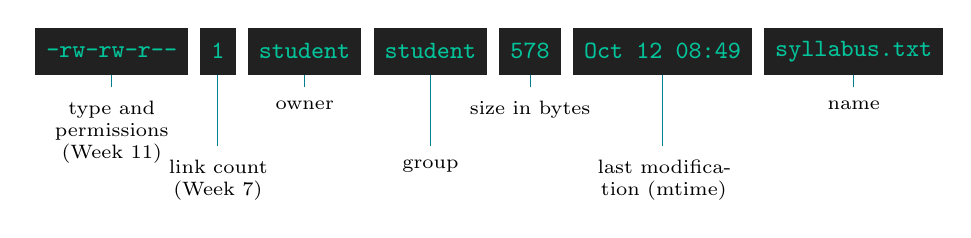
\begin{tikzpicture}[f/.style={rectangle,fill=dark,text=mint,font=\ttfamily\small,minimum height=0.6cm,inner sep=4pt},
  n/.style={font=\scriptsize,align=center,text width=1.9cm,anchor=north}]
\node[f] (a) at (0,0) {-rw-rw-r--};
\node[f,right=4pt of a] (b) {1};
\node[f,right=4pt of b] (c) {student};
\node[f,right=4pt of c] (d) {student};
\node[f,right=4pt of d] (e) {578};
\node[f,right=4pt of e] (g) {Oct 12 08:49};
\node[f,right=4pt of g] (h) {syllabus.txt};
\foreach \x/\t/\dy in {a/{type and permissions (Week 11)}/0,b/{link count (Week 7)}/0.75,c/owner/0,d/group/0.75,e/{size in bytes}/0,g/{last modification (mtime)}/0.75,h/name/0} {
  \draw[mintdeep] (\x.south) -- ++(0,-0.15-\dy);
  \node[n] at ($(\x.south)+(0,-0.2-\dy)$) {\t};}
\end{tikzpicture}
\caption{The seven columns of a line of \cmd{ls -l}.}
\label{fig:lsl}
\end{figure}

\begin{enumerate}[leftmargin=1.4em]
  \item \textbf{Type and permissions.} The first character is the type: \texttt{-} regular file, \texttt{d} directory, \texttt{l} symbolic link, \texttt{c} character device. The next nine characters are the read/write/execute permissions for the owner, the group and all others; Week~11 is devoted to them.
  \item \textbf{Link count.} For a file: the number of hard links (names) pointing to its inode (Week~7). For a directory: $2 + {}$the number of its subdirectories (see below).
  \item \textbf{Owner} and \textbf{group} of the file.
  \item \textbf{Size} in bytes. A directory shows the size of its own table of entries, usually one block of $4096$ bytes.
  \item \textbf{Modification time} (mtime): the last change of the \emph{contents}. Files older than six months show the year instead of the time (\texttt{Apr 22 2024} in Section~\ref{sec:fhs}).
  \item \textbf{Name.}
\end{enumerate}

\begin{keyidea}[ls -l shows the inode]
Apart from the name, every column of \cmd{ls -l} is a field of the file's \emph{inode} (Week~7): type, permissions, link count, owner, group, size and times. The name comes from the directory entry. Week~10 shows the complete inode with \cmd{stat}.
\end{keyidea}

\paragraph{Directory link counts.} Why does \texttt{projects} have link count $4$ and \texttt{docs} only $2$? A directory is named by its entry in the parent directory, by its own entry \texttt{.}, and by the entry \texttt{..} inside each of its subdirectories. Hence
\[
\text{link count of a directory} = 2 + s,
\]
where $s$ is the number of subdirectories: \texttt{projects} has $s = 2$ (\texttt{alpha} and \texttt{beta}), so $2 + 2 = 4$; \texttt{docs} has $s=0$, so $2$. (Checked with \texttt{code/check\_numbers.py}.)

\paragraph{The \texttt{total} line.} The first line, \texttt{total 24}, is the disk space used by the listed files in units of $1$\,KiB. Even a $16$-byte file occupies a whole file-system block of $4$\,KiB, so six small files use $6 \times 4 = 24$\,KiB (the block idea of Week~7). In \texttt{\tl/lab} itself, \cmd{ls -l} shows \texttt{total 36}: nine entries, $9 \times 4 = 36$.

\subsection{Human-readable sizes: ls -lh}

\outl{out_ls.txt}{33}{42}

With \cmd{-h} the sizes are printed with the suffixes K, M, G, which here mean powers of $1024$: $1\,\text{K} = 2^{10} = 1024$ bytes, $1\,\text{M} = 2^{20}$ bytes. \cmd{ls} rounds \emph{up}, and shows one decimal for values below $10$:

\begin{example}[From bytes to ls -h]
\begin{align*}
\texttt{access.log}:&\quad 23\,604 / 1024 \approx 23.05 \ \longrightarrow\ \texttt{24K}\ (\text{rounded up})\\
\texttt{system.log}:&\quad 5\,207 / 1024 \approx 5.085 \ \longrightarrow\ \texttt{5.1K}\\
\texttt{students.csv}:&\quad 1\,208 / 1024 \approx 1.180 \ \longrightarrow\ \texttt{1.2K}
\end{align*}
Files smaller than $1024$ bytes (such as \texttt{cities.txt}, $227$ bytes) are shown in bytes. The exact byte counts come from \cmd{ls -l} (Lab Sheet, Exercise~B7).
\end{example}

\subsection{Whole subtrees: ls -R and tree}

\cmd{ls -R} (\emph{recursive}) lists a directory and then every subdirectory below it, one block per directory. The program \cmd{tree} draws the same information as a picture --- the tree of Week~7. (\cmd{tree} may need to be installed: \cmd{sudo apt install tree}.)

\outl{out_tree.txt}{2}{13}
\vspace{-0.4em}{\small\color{muted}\quad \ldots\ (the same for \texttt{projects/beta}; full output in \texttt{code/out\_tree.txt})}

\begin{tcolorbox}[enhanced,colback=dark,colframe=dark,arc=0pt,boxrule=0pt,left=6pt,right=6pt,top=4pt,bottom=4pt,coltext=light,fontupper=\footnotesize]
\begin{verbatim}
student@okan-lab:~/lab$ tree projects
projects
├── alpha
│   ├── README.md
│   ├── docs
│   │   └── design.txt
│   └── src
│       └── main.c
└── beta
    ├── README.md
    ├── docs
    │   └── design.txt
    └── src
        └── main.c

7 directories, 6 files
\end{verbatim}
\end{tcolorbox}

\cmd{tree} counts \texttt{projects} itself, hence ``7 directories''. \textbf{Careful:} \cmd{ls -R /} would list the entire file system --- hundreds of thousands of lines. Press \texttt{Ctrl+C} to stop a command that runs too long.

\subsection{The most useful ls options}

\begin{center}
\begin{tabularx}{\linewidth}{>{\ttfamily}l >{\raggedright\arraybackslash}X >{\ttfamily}l}
\toprule
\normalfont\textbf{Option} & \textbf{Meaning} & \normalfont\textbf{Example}\\
\midrule
-l & long listing (Figure~\ref{fig:lsl}) & ls -l docs\\
-a / -A & all names, including hidden ones (-A: without \texttt{.} and \texttt{..}) & ls -a \tl\\
-h & human-readable sizes (with -l) & ls -lh logs\\
-R & recursive: also every subdirectory & ls -R projects\\
-F & mark type: \texttt{/} directory, \texttt{*} executable, \texttt{@} link & ls -F\\
-d & the directory itself, not its contents & ls -ld projects\\
-S & sort by size, largest first & ls -lS docs\\
-t & sort by modification time, newest first & ls -lt\\
-r & reverse the sort order & ls -ltr\\
-1 & one name per line & ls -1 photos\\
-i & show inode numbers (Week 7) & ls -i\\
\bottomrule
\end{tabularx}
\end{center}
Ubuntu's default \texttt{\tl/.bashrc} also defines the shortcuts (\emph{aliases}) \cmd{ll} $=$ \cmd{ls -alF}, \cmd{la} $=$ \cmd{ls -A} and \cmd{l} $=$ \cmd{ls -CF}.

% =====================================================================
\section{The Linux Directory Tree}
\label{sec:fhs}

Linux has \emph{one} tree with \emph{one} root, \texttt{/}. There are no drive letters: other disks and USB sticks are \emph{mounted} into the tree (typically under \texttt{/media} or \texttt{/mnt}). The \term{Filesystem Hierarchy Standard} (FHS) says which directory holds what, so that all distributions look alike.

\begin{figure}[H]
\centering
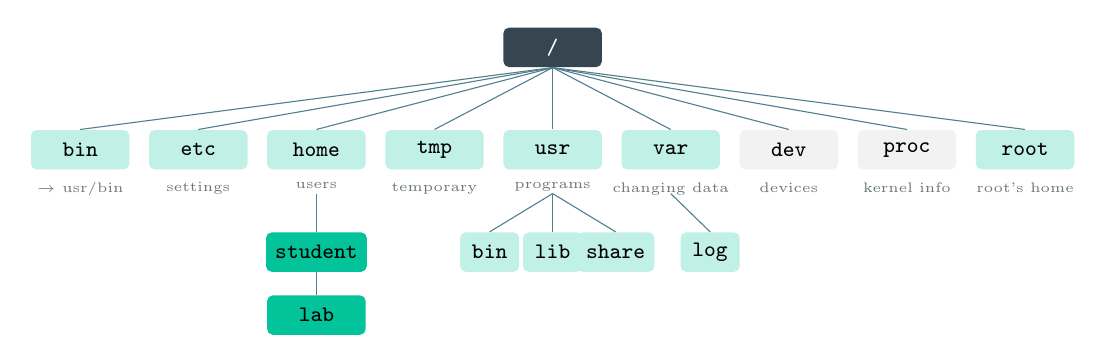
\begin{tikzpicture}[d/.style={rectangle,rounded corners=2pt,fill=mint!25,minimum width=1.25cm,minimum height=0.5cm,font=\footnotesize\ttfamily},
  v/.style={d,fill=light}, s/.style={font=\tiny,text=muted,align=center}]
\node[d,fill=charcoal,text=white] (r) at (6.0,0) {/};
\foreach \n/\t/\st [count=\i from 0] in {bin/{$\to$ usr/bin}/d,etc/settings/d,home/users/d,tmp/temporary/d,usr/programs/d,var/{changing data}/d,dev/devices/v,proc/{kernel info}/v,root/{root's home}/d} {
  \node[\st] (n\i) at (1.5*\i,-1.3) {\n};
  \node[s,below=1pt of n\i] {\t};
  \draw[slate] (r.south) -- (n\i.north);
}
\node[d,fill=mint] (st) at (3.0,-2.6) {student}; \draw[slate] (n2.south) ++(0,-0.3) -- (st.north);
\node[d,fill=mint] (lab) at (3.0,-3.4) {lab}; \draw[slate] (st) -- (lab);
\foreach \n/\x in {bin/5.2,lib/6.0,share/6.8} { \node[d,minimum width=0.75cm] (u\n) at (\x,-2.6) {\n}; \draw[slate] (n4.south) ++(0,-0.3) -- (u\n.north); }
\node[d,minimum width=0.75cm] (vl) at (8.0,-2.6) {log}; \draw[slate] (n5.south) ++(0,-0.3) -- (vl.north);
\end{tikzpicture}
\caption{The top of the Linux directory tree. Grey: virtual file systems generated by the kernel.}
\end{figure}

\begin{center}
\begin{tabularx}{\linewidth}{>{\ttfamily}l >{\raggedright\arraybackslash}X >{\ttfamily\raggedright\arraybackslash}p{4.1cm}}
\toprule
\normalfont\textbf{Directory} & \textbf{Contents} & \normalfont\textbf{Try}\\
\midrule
/ & the root of the whole tree & ls /\\
/home & one home directory per user: \texttt{/home/student} & ls \tl\\
/root & home directory of the administrator \texttt{root} (not the same as \texttt{/}) & ---\\
/etc & system-wide configuration, mostly plain text files & head -n 4 /etc/os-release\\
/usr & installed software: \texttt{/usr/bin} programs, \texttt{/usr/lib} libraries, \texttt{/usr/share} data & ls -l /usr/bin/ls\\
/bin, /sbin, /lib & on Ubuntu 24.04 symbolic links to \texttt{/usr/bin}, \texttt{/usr/sbin}, \texttt{/usr/lib} & ls -ld /bin\\
/var & variable data that grows: logs (\texttt{/var/log}), caches, mail, spool & ls /var\\
/tmp & temporary files; everyone may write; often emptied at boot & ls -ld /tmp\\
/dev & device files: disks, terminals, \texttt{/dev/null} & ls -l /dev/null\\
/proc & virtual: information about processes and the kernel, generated on the fly & head /proc/meminfo\\
/media, /mnt & mount points for removable and other disks & ---\\
/boot & the kernel image and boot loader files & ---\\
\bottomrule
\end{tabularx}
\end{center}

\subsection{A tour}

In the listing of \texttt{/} below, two entries that exist only on our test machine have been left out. The directories ending in \texttt{.usr-is-merged} are a harmless leftover of Ubuntu's move to a ``merged \texttt{/usr}''.

\outl{out_fhs.txt}{1}{23}

\begin{itemize}
  \item \cmd{type ls} reveals that \cmd{ls} is simply a program file, \texttt{/usr/bin/ls} ($142\,312$ bytes). Most commands are files like this.
  \item \texttt{/bin}, \texttt{/sbin} and \texttt{/lib} are \term{symbolic links} (type \texttt{l}, arrow \texttt{->}; Week~7) to their counterparts in \texttt{/usr}. Both names lead to the same programs.
  \item \texttt{/etc/os-release} names the distribution. UNIX keeps configuration as editable text; Week~11 reads \texttt{/etc/passwd} and \texttt{/etc/group}.
  \item \texttt{/tmp} has permission string \texttt{drwxrwxrwt}: everyone may create files there, and the final \texttt{t} (the \emph{sticky bit}, Week~11) stops users from deleting each other's files.
\end{itemize}

\subsection{/dev and /proc: everything is a file}

\outl{out_fhs.txt}{24}{41}

\begin{itemize}
  \item In \texttt{/dev}, the \texttt{c} marks \emph{character devices}. Instead of a size, \cmd{ls -l} shows two driver numbers (major, minor), e.g.\ \texttt{1, 3}. \texttt{/dev/null} discards everything written to it (we used it with \cmd{strace}); \texttt{/dev/zero} produces zero bytes; \texttt{/dev/tty} is your terminal. Programs use these devices with the same \texttt{open/read/write} system calls as ordinary files (Week~2, I/O).
  \item \texttt{/proc} is not stored on any disk. When you read one of its files, the kernel writes the text on the fly. \texttt{/proc/meminfo} shows that our test machine has about $8$\,GB of RAM ($8\,222\,320$\,kB).
  \item \texttt{\$\$} is replaced by the shell with its own PID. \texttt{/proc/<PID>/status} shows part of that process's PCB (Week~3): its name (\texttt{bash}), state \texttt{S} (sleeping --- it is waiting for \cmd{head} to finish), PID and parent PID (\texttt{PPid}). Week~13 returns to \texttt{/proc} and \cmd{ps}.
\end{itemize}

% =====================================================================
\section{Moving Around: cd and Paths}
\label{sec:paths}

\subsection{Absolute and relative paths}

As in Week~7, a file or directory can be named in two ways:
\begin{itemize}
  \item An \term{absolute path} starts with \texttt{/} and walks down from the root. It means the same thing from anywhere: \texttt{/home/student/lab/projects/beta/docs}.
  \item A \term{relative path} does not start with \texttt{/}; it walks from the current directory. \texttt{..} means ``one level up''.
\end{itemize}

\begin{figure}[H]
\centering
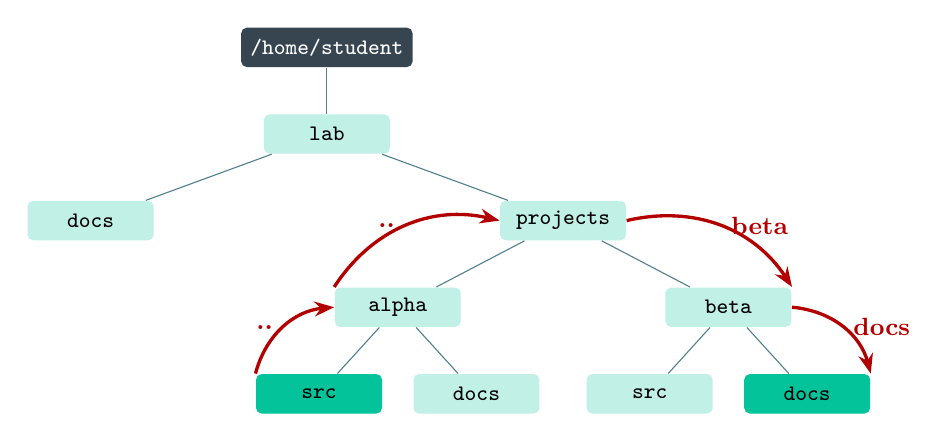
\begin{tikzpicture}[level distance=1.1cm,
  dir/.style={rectangle,rounded corners=2pt,fill=mint!25,minimum width=1.6cm,minimum height=0.5cm,font=\footnotesize\ttfamily},
  level 1/.style={sibling distance=5.5cm}, level 2/.style={sibling distance=6cm}, level 3/.style={sibling distance=4.2cm}, level 4/.style={sibling distance=2.0cm},
  edge from parent/.style={draw,slate},
  r/.style={-{Stealth[length=2.5mm]},very thick,red!70!black}]
\node[dir,fill=charcoal,text=white] {/home/student}
  child {node[dir] {lab}
    child {node[dir] {docs}}
    child {node[dir] (pr) {projects}
      child {node[dir] (al) {alpha} child {node[dir,fill=mint] (as) {src}} child {node[dir] {docs}}}
      child {node[dir] (be) {beta} child {node[dir] {src}} child {node[dir,fill=mint] (bd) {docs}}}}};
\draw[r] (as.north west) to[bend left=35] node[left,font=\small\bfseries]{..} (al.west);
\draw[r] (al.north west) to[bend left=35] node[left,font=\small\bfseries]{..} (pr.west);
\draw[r] (pr.east) to[bend left=35] node[right,font=\small\bfseries]{beta} (be.north east);
\draw[r] (be.east) to[bend left=35] node[right,font=\small\bfseries]{docs} (bd.north east);
\end{tikzpicture}
\caption{From \texttt{projects/alpha/src} to \texttt{projects/beta/docs}: \texttt{../../beta/docs} (up, up, down, down).}
\label{fig:paths}
\end{figure}

\subsection{cd in practice}

\outl{out_cd.txt}{1}{22}

What to observe:
\begin{itemize}
  \item The prompt shows the new current directory after every \cmd{cd}.
  \item \cmd{cd} prints \emph{nothing} when it succeeds (``no news is good news'' is a UNIX rule). The only exception is \cmd{cd -}, which prints the directory it jumps back to.
  \item \cmd{cd ../../docs} from \texttt{\tl/lab/projects/alpha} goes up twice (to \texttt{\tl/lab}) and then down into \texttt{docs}.
  \item The absolute path \texttt{/home/student/lab/projects/beta} works no matter where you are.
  \item \cmd{cd} without an argument takes you home; \cmd{cd /} to the root.
\end{itemize}

\subsection{Five special names}

\begin{center}
\begin{tabularx}{\linewidth}{>{\ttfamily}l >{\raggedright\arraybackslash}X >{\ttfamily}l >{\raggedright\arraybackslash}p{5.3cm}}
\toprule
\normalfont\textbf{Name} & \textbf{Meaning} & \normalfont\textbf{Example} & \textbf{Result from \texttt{\tl/lab/projects/alpha}}\\
\midrule
/ & the root of the tree & cd / & \texttt{/}\\
\tl & your home directory & cd \tl/lab & \texttt{/home/student/lab}\\
. & the current directory & ls . & lists \texttt{alpha} (same as \cmd{ls})\\
.. & the parent directory & cd ../beta & \texttt{\tl/lab/projects/beta}\\
- & the previous directory (\cmd{cd} only) & cd - & back to where you were\\
\bottomrule
\end{tabularx}
\end{center}
\texttt{.} and \texttt{..} are real directory entries (\cmd{ls -a} shows them); \texttt{\tl} and \texttt{-} are shortcuts of the shell: \texttt{\tl} is replaced by the value of \texttt{\$HOME}, and \cmd{cd -} uses the variable \texttt{\$OLDPWD}, as \cmd{help cd} explains (Section~\ref{sec:help}). The \texttt{..} of \texttt{/} is \texttt{/} itself: you cannot go above the root. The name \texttt{.} becomes important in Weeks~11 and~14: \texttt{./script.sh} runs a script from the current directory.

\subsection{Why cd must be a shell builtin}
\label{sec:cdbuiltin}

\outl{out_syscalls.txt}{8}{18}

\begin{itemize}
  \item \texttt{/bin/pwd} is a separate program (not the builtin \cmd{pwd}); it asks the kernel for the current directory with the system call \texttt{getcwd}. It prints \texttt{/home/student/lab}: a child inherits the current directory of its parent.
  \item \cmd{bash -c 'cd /tmp'} starts a \emph{child} shell that runs \cmd{cd /tmp}. The kernel call \texttt{chdir("/tmp")} succeeds --- but afterwards our own shell is still in \texttt{\tl/lab}.
\end{itemize}

\begin{keyidea}[The current directory belongs to the process]
The current working directory is part of the state the kernel keeps for each process, next to its PCB (Week~3). A process can change only its \emph{own} current directory, never its parent's. If \cmd{cd} were a program in \texttt{/usr/bin}, the shell would fork a child, the child would change \emph{its} directory and exit --- and the shell would stay where it was. Therefore \cmd{cd} is built into the shell: \cmd{bash} calls \texttt{chdir()} on itself. \cmd{type cd} confirms: ``cd is a shell builtin''. The same argument applies to \cmd{exit} and to commands that set shell variables.
\end{keyidea}

% =====================================================================
\section{Getting Help}
\label{sec:help}

Nobody remembers every option. Know where to look:

\begin{description}[leftmargin=0pt,itemsep=0.25em]
  \item[\cmd{command --help}] A summary of the options, printed by most programs.
  \item[\cmd{man command}] The full \emph{manual page}, divided into sections such as NAME, SYNOPSIS, DESCRIPTION, OPTIONS and EXAMPLES. Move with the arrow keys or Space (next page), search with \texttt{/word} and Enter (\texttt{n} for the next match), quit with \texttt{q}. \cmd{man man} explains \cmd{man} itself.
  \item[\cmd{help command}] Help for shell builtins (\cmd{cd}, \cmd{pwd}, \cmd{history}), which have no program file and often no manual page of their own.
  \item[\cmd{type command}] Tells whether a command is a builtin, an alias or a program file (and where).
  \item[\cmd{whatis} / \cmd{apropos}] \cmd{whatis ls} prints the one-line description from the manual; \cmd{apropos directory} searches all manual descriptions for a keyword --- useful when you do not know the command's name.
  \item[\cmd{tldr command}] (optional, \cmd{sudo apt install tldr}) community-written short examples of common uses.
\end{description}

\outl{out_help.txt}{1}{8}
\outl{out_help.txt}{14}{23}

Reading a SYNOPSIS: \texttt{ls [OPTION]... [FILE]...} means ``any number of options, then any number of files, all optional'' --- square brackets mark optional parts and \texttt{...} means ``may be repeated''. The output of \cmd{ls --help} was shortened with \texttt{| head -n 12} (only the first $12$ lines; pipes are the topic of Week~12).

Our test machine is a \emph{minimised} Ubuntu without manual pages, which is why these notes show \cmd{--help} output instead of \cmd{man} output; normal installations, WSL and the lab PCs have them (\cmd{sudo unminimize} restores them on a minimised system).

% =====================================================================
\section{Working Smarter: Completion, History, Shortcuts}

\subsection{Tab completion}
Press \texttt{Tab} after the first letters of a command, file or directory name and the shell completes it. In the session below, the user typed \texttt{cd pro}\,\texttt{Tab}\,\texttt{al}\,\texttt{Tab} and the shell completed it to \texttt{cd projects/alpha/}; \texttt{ls \tl/lab/docs/sy}\,\texttt{Tab} became \texttt{ls \tl/lab/docs/syllabus.txt} (with a space added after the complete name). If the beginning is ambiguous (\texttt{notes\_0} could be three files), nothing seems to happen: press \texttt{Tab} \emph{twice} to see the list of candidates. Tab completion saves typing \emph{and} prevents typing errors.

\subsection{History}

\outl{out_keys.txt}{1}{24}

The shell remembers your commands. \cmd{history} prints them with numbers; \cmd{!!} repeats the last command and \cmd{!5} repeats command number~$5$ (the shell first prints the command it is going to run). The arrow keys \texttt{↑}/\texttt{↓} walk through the history, and \texttt{Ctrl+R} searches it backwards as you type. The history is saved in the file \texttt{\tl/.bash\_history} when the shell exits.

\subsection{Keyboard shortcuts}

\begin{center}
\begin{tabular}{>{\ttfamily}l l}
\toprule
\normalfont\textbf{Key} & \textbf{Effect}\\
\midrule
Tab / Tab Tab & complete a name / list the candidates\\
↑ / ↓ & previous / next command from the history\\
Ctrl+R & search the history backwards\\
Ctrl+C & interrupt (stop) the running command --- it sends the signal SIGINT (Week 13)\\
Ctrl+L & clear the screen (like \cmd{clear})\\
Ctrl+A / Ctrl+E & jump to the beginning / end of the line\\
Ctrl+D & end of input; at an empty prompt it closes the shell (like \cmd{exit})\\
\bottomrule
\end{tabular}
\end{center}
Copy and paste in most terminal windows use \texttt{Ctrl+Shift+C} and \texttt{Ctrl+Shift+V}, because \texttt{Ctrl+C} already means ``interrupt''.

% =====================================================================
\section{Command Reference: Week 9}

\begin{center}
\begin{tabularx}{\linewidth}{>{\ttfamily\raggedright\arraybackslash}p{3.6cm} >{\raggedright\arraybackslash}X}
\toprule
\normalfont\textbf{Command} & \textbf{Purpose}\\
\midrule
whoami & print your user name\\
hostname & print the computer's name\\
date & print the date and time\\
echo text & print its arguments (after the shell has expanded them)\\
uname [-r|-a] & kernel name / release / all information\\
clear & clear the screen (\texttt{Ctrl+L})\\
pwd & print the current working directory (absolute path)\\
ls [-laAhRFdStr1i] [dir...] & list directory contents (Section~\ref{sec:ls})\\
tree [dir] & draw a directory tree\\
cd [dir] & change directory; \texttt{\tl\ . .. - /}; no argument: home\\
cat file & print a small file (Week 10 covers \cmd{cat}, \cmd{less}, \cmd{head}, \cmd{tail})\\
head -n N file & print the first $N$ lines of a file\\
type cmd & builtin, alias or program file?\\
cmd --help & short help of a program\\
man cmd & manual page (\texttt{q} quits, \texttt{/word} searches)\\
help cmd & help for a shell builtin\\
whatis cmd / apropos word & one-line description / search the manuals\\
history, !!, !n & list / repeat previous commands\\
strace cmd & show the system calls of a command (Week 2)\\
bash file.sh & run a shell script (e.g.\ the lab setup script)\\
\bottomrule
\end{tabularx}
\end{center}

% =====================================================================
\section{Common Errors and What They Mean}
\label{sec:errors}

Error messages are precise; read them. All of the following were produced in \texttt{\tl/lab}:

\outl{out_errors.txt}{2}{27}

\begin{description}[leftmargin=0pt,itemsep=0.25em]
  \item[\texttt{command not found}] A typing error, the wrong case (\cmd{LS}), or a program that is not installed (\cmd{sl}). On a normal Ubuntu the shell also suggests a package, e.g.\ ``Command 'sl' not found, but can be installed with: sudo apt install sl''.
  \item[\texttt{invalid option}] The command does not have this option. The message itself suggests \cmd{ls --help}.
  \item[\texttt{No such file or directory}] The name is wrong (remember case: \texttt{Docs} $\neq$ \texttt{docs}), or you are not in the directory you think you are in. Run \cmd{pwd} and \cmd{ls}, and use Tab completion.
  \item[\texttt{Not a directory}] \cmd{cd} needs a directory; \texttt{README.txt} is a file.
  \item[Two errors for one name] The shell splits a command line at spaces, so \texttt{docs/final report.txt} becomes \emph{two} arguments, \texttt{docs/final} and \texttt{report.txt}. Put the name in quotes (\texttt{"docs/final report.txt"}) or escape the space with a backslash (\texttt{docs/final\textbackslash\ report.txt}). With \cmd{cd}, two arguments give \texttt{too many arguments}.
  \item[\texttt{Permission denied}] You are not allowed in (\texttt{/root} belongs to the administrator). This is the protection system working as designed (Week~11). Do \emph{not} react by putting \cmd{sudo} in front of commands.
  \item[\texttt{\$'\textbackslash r': command not found}] A script with Windows line endings (Section~\ref{sec:labsetup}).
\end{description}

\begin{tryit}[A word on sudo]
\cmd{sudo} runs one command as \texttt{root}, the administrator, after asking for \emph{your} password. In this course you need it only to install software (\cmd{sudo apt install tree}). As \texttt{root}, the protection mechanisms of Weeks~2 and~11 no longer protect you from your own mistakes: one wrong command can damage the system. Never use \cmd{sudo} just because a command failed.
\end{tryit}

% =====================================================================
\section{Summary}

\begin{keyidea}[Week 9 in seven sentences]
\begin{enumerate}[leftmargin=1.4em]
  \item A Linux shell is available on the lab PCs, with WSL on Windows (\cmd{wsl --install}) or in a VirtualBox VM; the script \texttt{mcmp117\_lab\_setup.sh} creates the practice folder \texttt{\tl/lab}.
  \item The terminal shows text, the shell (\cmd{bash}) interprets commands in user mode, and the kernel does the work through system calls.
  \item For an external command the shell forks, the child execs the program file, and the shell waits (Week~3); builtins such as \cmd{cd} run inside the shell.
  \item A command line has the form \emph{command -options arguments}; words are separated by spaces and case matters.
  \item \cmd{pwd} shows where you are; \cmd{ls} (with \cmd{-l -a -h -R -F}) shows what is there; \cmd{ls -l} displays the inode fields of Week~7.
  \item Linux has one tree from \texttt{/}; \cmd{cd} moves with absolute or relative paths and the names \texttt{\tl\ . .. -}.
  \item \cmd{--help}, \cmd{man}, \cmd{help} and \cmd{type} explain commands; Tab, history and \texttt{Ctrl+C}/\texttt{Ctrl+L} save time.
\end{enumerate}
\end{keyidea}

% =====================================================================
\Needspace{12\baselineskip}
\section{Glossary}

\begin{description}[leftmargin=0pt,itemsep=0.15em]
  \item[Absolute path] A path starting at the root \texttt{/}; valid from any directory.
  \item[Builtin] A command executed by the shell itself, without a new process (\cmd{cd}, \cmd{pwd}, \cmd{echo}, \cmd{history}).
  \item[Current working directory] The directory from which a process resolves relative paths; part of each process's state.
  \item[FHS] Filesystem Hierarchy Standard: which top-level directory holds what.
  \item[Hidden file] A file whose name starts with a dot; shown only by \cmd{ls -a}.
  \item[Home directory] A user's own directory, \texttt{/home/<user>}, abbreviated \texttt{\tl}.
  \item[Option] A word starting with \texttt{-} or \texttt{--} that changes how a command works.
  \item[Prompt] The text the shell prints when it is ready for a command.
  \item[Relative path] A path starting from the current directory; may use \texttt{..}.
  \item[Shell] The command interpreter: a user-mode system program that reads commands and runs them.
  \item[Terminal (emulator)] The window program that passes keystrokes to the shell and displays its output.
  \item[WSL] Windows Subsystem for Linux: runs a Linux distribution with a real Linux kernel inside Windows.
\end{description}

% =====================================================================
\section{Lab Sheet}
\label{sec:lab}

Re-create the lab folder first (\cmd{bash mcmp117\_lab\_setup.sh}), then start every exercise in \texttt{\tl/lab} unless stated otherwise. Write down the \emph{commands} you used and the answers. Total: $100$ points. Solutions are in Section~\ref{sec:labsol} --- try first! In this lab you may use \cmd{cat file} to print a small file and \cmd{head -n N file} to print its first $N$ lines.

\subsection*{Part A --- Getting started (13 points)}
\begin{enumerate}[label=\textbf{A\arabic*}, leftmargin=2.2em]
  \item \textbf{(4 pts)} Run \cmd{whoami}, \cmd{hostname}, \cmd{date} and \cmd{uname -r}. Write down the output and say in one sentence what each command reports.
  \item \textbf{(4 pts)} Run the lab setup script. What is the \emph{absolute} path of your lab folder? Which command proves it?
  \item \textbf{(5 pts)} For each command line, name the command, the options and the arguments: (a) \cmd{ls -l -a docs}, (b) \cmd{ls -lh /var/log /tmp}, (c) \cmd{head -n 3 data/cities.txt}, (d) \cmd{cd}, (e) \cmd{ls --all}.
\end{enumerate}

\subsection*{Part B --- Looking around (30 points)}
\begin{enumerate}[label=\textbf{B\arabic*}, leftmargin=2.2em, start=4]
  \item \textbf{(6 pts)} How many entries does \cmd{ls} show in \texttt{\tl/lab}? How many of them are directories? Which option makes the answer obvious?
  \item \textbf{(6 pts)} \texttt{docs} contains a hidden file. Find its name and print its contents.
  \item \textbf{(6 pts)} Which file in \texttt{docs} is the largest, and how many bytes does it have? Use the option of \cmd{ls} that sorts by size (find it in \cmd{ls --help}).
  \item \textbf{(6 pts)} Give the exact size of \texttt{logs/access.log} in bytes and the size shown by \cmd{ls -lh}. Show by calculation why they agree.
  \item \textbf{(6 pts)} How many files are in \texttt{photos}? How many of them end exactly in \texttt{.jpg} (lower case)? Which do not?
\end{enumerate}

\subsection*{Part C --- Moving around (24 points)}
\begin{enumerate}[label=\textbf{C\arabic*}, leftmargin=2.2em, start=9]
  \item \textbf{(6 pts)} From \texttt{\tl/lab}, go to \texttt{projects/beta/docs} with \emph{one} relative \cmd{cd} and print the current directory.
  \item \textbf{(6 pts)} From there, go to \texttt{projects/alpha/src} with one relative \cmd{cd}. Write the command and check with \cmd{pwd}.
  \item \textbf{(6 pts)} Starting in \texttt{\tl/lab/projects}, you type \cmd{cd alpha}, \cmd{cd ../beta/src}, \cmd{cd ..}, \cmd{cd -}. \emph{Predict} the directory after each command, then check.
  \item \textbf{(6 pts)} Write two different commands that take you to \texttt{\tl/lab/src} \emph{from any directory}. Why does \cmd{cd lab/src} work only in some directories?
\end{enumerate}

\subsection*{Part D --- The system and help (18 points)}
\begin{enumerate}[label=\textbf{D\arabic*}, leftmargin=2.2em, start=13]
  \item \textbf{(6 pts)} Where is the program \cmd{ls} stored? What exactly is \texttt{/bin} on Ubuntu 24.04? Which file tells you the name and version of the distribution, and what does it say on your system?
  \item \textbf{(6 pts)} Print the PID of your shell and the lines \texttt{Name}, \texttt{State}, \texttt{Pid} and \texttt{PPid} of \texttt{/proc/<PID>/status}. Which data structure of Week~3 is this a view of, and why is the state \texttt{S}?
  \item \textbf{(6 pts)} Using \cmd{ls --help}, find the option that lists one name per line and the option that reverses the sort order. Use both together on \texttt{docs}. Then use \cmd{help cd} to explain what \cmd{cd -} does.
\end{enumerate}

\subsection*{Part E --- Challenges (15 points)}
\begin{enumerate}[label=\textbf{E\arabic*}, leftmargin=2.2em, start=16]
  \item \textbf{(5 pts) Treasure hunt.} Start in \texttt{\tl/lab} and use only \cmd{cd}, \cmd{ls}, \cmd{pwd} and \cmd{cat}. (1) Read \texttt{README.txt}: go to the directory that holds ``a small C program''. (2) What does that program print? (3) With one relative \cmd{cd}, move to the directory of short text documents. (4) One file there has a space in its name; its last line is the password. (5) Finish in \texttt{projects/beta/src} with one relative \cmd{cd} and run \cmd{pwd}.
  \item \textbf{(5 pts) Link counts.} \cmd{ls -ld} shows link count $10$ for \texttt{\tl/lab}, $4$ for \texttt{projects} and for \texttt{projects/alpha}, and $2$ for \texttt{docs}. Explain all four numbers with the Week~7 idea of hard links, and predict the link count of \texttt{projects/beta}.
  \item \textbf{(5 pts) Why a builtin?} Run \cmd{type cd}, \cmd{strace -e trace=chdir bash -c 'cd /tmp'} and then \cmd{pwd}. Explain, using the process concept of Week~3, why \cmd{cd} cannot be an ordinary program.
\end{enumerate}

% =====================================================================
\section{Review Questions}

\subsection*{Conceptual}
\begin{enumerate}[leftmargin=1.6em]
  \item Explain the difference between a terminal, a shell and the kernel. Which of them run in user mode?
  \item List the steps the shell takes when you type \cmd{ls docs}. Which system calls of Week~3 are involved?
  \item What is the difference between a builtin and an external command? How can you tell which one a command is?
  \item What is a hidden file? How do you list hidden files?
  \item Explain each column of the line \texttt{drwxrwxr-x 4 student student 4096 Oct 12 08:49 projects}.
  \item Why does Linux not need drive letters? What is \texttt{/proc}, and why is it called a virtual file system?
  \item Explain the difference between an absolute and a relative path, with one example of each that names the same directory.
  \item What do \texttt{\tl}, \texttt{.}, \texttt{..} and \texttt{-} mean for \cmd{cd}? Which of them are real directory entries?
  \item Why does \cmd{ls docs/final report.txt} print two error messages? Give two ways to fix the command.
\end{enumerate}

\subsection*{Numerical}
\begin{enumerate}[leftmargin=1.6em,resume]
  \item A file has $3\,500\,000$ bytes. What does \cmd{ls -lh} show?
  \item A file has $10\,300$ bytes. What does \cmd{ls -lh} show?
  \item A directory has $5$ subdirectories and $12$ files. What is its link count?
  \item A directory contains $7$ files, each smaller than $4$\,KiB, and the file system uses $4$\,KiB blocks. What does the \texttt{total} line of \cmd{ls -l} show?
  \item You are in \texttt{/home/student/lab/projects/alpha/docs}. Write the shortest relative path to \texttt{/home/student/lab/data}. How many levels up does it go?
\end{enumerate}

\subsection*{Answers to the numerical questions}
\begin{enumerate}[leftmargin=1.6em,start=10]
  \item $3\,500\,000 / 2^{20} = 3\,500\,000 / 1\,048\,576 \approx 3.338$; one decimal, rounded up: \texttt{3.4M}.
  \item $10\,300 / 1024 \approx 10.06$; at $10$ or more no decimal is shown and the value is rounded up: \texttt{11K}.
  \item $2 + 5 = 7$ (files do not count).
  \item Each file occupies one block: $7 \times 4 = 28$, so \texttt{total 28}.
  \item \texttt{../../../data}: up three levels (to \texttt{docs}' parent \texttt{alpha}, then \texttt{projects}, then \texttt{lab}), then down into \texttt{data}.
\end{enumerate}

% =====================================================================
\section{Lab Sheet Solutions}
\label{sec:labsol}

The outputs below are from \texttt{code/out\_lab.txt} (script \texttt{code/demo\_lab.sh}) and the other transcripts of this week. Dates, PIDs and system details will differ on your computer.

\paragraph{A1.} See Section~\ref{sec:first}: \texttt{student}, \texttt{okan-lab}, the current date and time, and the kernel release (\texttt{6.18.44-fc-v114} on our machine). \cmd{whoami}: user name; \cmd{hostname}: computer name; \cmd{date}: date and time; \cmd{uname -r}: version of the Linux kernel.

\paragraph{A2.} The script prints \texttt{Lab folder ready: /home/student/lab} (Section~\ref{sec:labsetup}). \cmd{cd \tl/lab} followed by \cmd{pwd} prints the absolute path \texttt{/home/student/lab} (with your own user name).

\paragraph{A3.} (a) command \cmd{ls}, options \texttt{-l -a}, argument \texttt{docs}; (b) \cmd{ls}, options \texttt{-l -h} (combined), arguments \texttt{/var/log} and \texttt{/tmp}; (c) \cmd{head}, option \texttt{-n} with value \texttt{3}, argument \texttt{data/cities.txt}; (d) \cmd{cd}, no options, no arguments (goes home); (e) \cmd{ls}, long option \texttt{--all}, no arguments.

\paragraph{B4.} $9$ entries: $8$ directories and the file \texttt{README.txt}. \cmd{ls -F} marks directories with \texttt{/} (\cmd{ls -l} shows \texttt{d}).

\paragraph{B5.} \cmd{ls -a docs} reveals \texttt{.settings}; \cmd{cat docs/.settings} prints \texttt{editor=nano} and \texttt{color=on}.

\paragraph{B6.} \cmd{-S} sorts by size, largest first: \cmd{ls -lS docs} puts \texttt{syllabus.txt} ($578$ bytes) at the top, followed by \texttt{linux\_quotes.txt} ($302$) and \texttt{final report.txt} ($53$).

\paragraph{B7.} \cmd{ls -l logs} gives $23\,604$ bytes; \cmd{ls -lh} shows \texttt{24K}, because $23\,604/1024 \approx 23.05$ and \cmd{ls -h} rounds up.

\paragraph{B8.} $15$ files. $12$ end in \texttt{.jpg} (\texttt{img001.jpg} \ldots\ \texttt{img012.jpg}); the other three are \texttt{IMG\_014.JPG} (upper case --- a different name on Linux), \texttt{holiday.jpeg} and \texttt{img013.png}. (Next week, wildcards such as \texttt{*.jpg} will count them for you.) \cmd{ls photos} shows all $15$ names in three columns.

\paragraph{C9 and C10.} \cmd{cd projects/beta/docs}, then \cmd{cd ../../alpha/src} (up to \texttt{beta}, up to \texttt{projects}, down to \texttt{alpha/src}); \cmd{pwd} prints \texttt{/home/student/lab/projects/beta/docs} and then \texttt{/home/student/lab/projects/alpha/src}.

\paragraph{C11.} After \cmd{cd alpha}: \texttt{\tl/lab/projects/alpha}; after \cmd{cd ../beta/src}: \texttt{\tl/lab/projects/beta/src}; after \cmd{cd ..}: \texttt{\tl/lab/projects/beta}; \cmd{cd -} returns to \texttt{\tl/lab/projects/beta/src} and prints it:

\paragraph{C12.} \cmd{cd /home/student/lab/src} (absolute; use your own user name) and \cmd{cd \tl/lab/src} (the shell expands \texttt{\tl} to the absolute path of your home). \cmd{cd lab/src} is relative: it works only when the current directory is \texttt{/home/student}, the directory that contains \texttt{lab}.

\paragraph{D13.} \cmd{type ls} $\to$ \texttt{/usr/bin/ls}; \cmd{ls -ld /bin} $\to$ a symbolic link to \texttt{usr/bin}; \texttt{/etc/os-release} names the distribution; on our machine \texttt{PRETTY\_NAME="Ubuntu 24.04.4 LTS"} (Section~\ref{sec:fhs}).

\paragraph{D14.} \cmd{echo \$\$}, then \cmd{head -n 7 /proc/\$\$/status} (Section~\ref{sec:fhs}; the PID differs every time). It is a view of the shell's \emph{process control block} (Week~3): name, state, PID, parent PID. The state is \texttt{S} (sleeping) because, while \cmd{head} runs, the shell is blocked in \texttt{wait()} for its child.

\paragraph{D15.} \cmd{-1} (one per line) and \cmd{-r} (reverse):
\outl{out_lab.txt}{64}{70}
\cmd{help cd} says: \emph{If DIR is ``-'', it is converted to \$OLDPWD}, i.e.\ \cmd{cd -} goes to the previous directory (Section~\ref{sec:help}).

\paragraph{E16 (treasure hunt).} (1) \texttt{README.txt} says \texttt{src/} holds ``a small C program'': \cmd{cd src}. (2) \cmd{cat hello.c}: the program prints \texttt{Hello from the lab!}. (3) \cmd{cd ../docs}. (4) \cmd{cat "final report.txt"}: the password is \texttt{This file name contains a space.} (5) \cmd{cd ../projects/beta/src}; \cmd{pwd} prints \texttt{/home/student/lab/projects/beta/src}.

\paragraph{E17.} Link count of a directory $= 2 + s$ ($s$ = number of subdirectories): its name in the parent, its own \texttt{.}, and one \texttt{..} in each subdirectory. \texttt{\tl/lab}: $s = 8$, $2+8 = 10$; \texttt{projects}: \texttt{alpha}, \texttt{beta}, $2+2 = 4$; \texttt{alpha}: \texttt{docs}, \texttt{src}, $4$; \texttt{docs}: $2$. Prediction for \texttt{projects/beta}: $4$.
\outl{out_lab.txt}{71}{75}

\paragraph{E18.} See Section~\ref{sec:cdbuiltin}: \cmd{type cd} prints ``cd is a shell builtin''; the child \cmd{bash} successfully calls \texttt{chdir("/tmp")}, but \cmd{pwd} afterwards still prints \texttt{/home/student/lab}. The current directory is per-process state; a child cannot change its parent's, so \cmd{cd} must run inside the shell process itself.

\paragraph{Grading hints.} Give full points when the commands are correct even if dates, PIDs and system details differ. In C9--C12 and E16, deduct points if absolute paths are used where a relative path was required.

% =====================================================================
\section{Looking Ahead: Week 10}

Next week we stop just looking and start \emph{changing} the file system in \texttt{\tl/lab}:
\begin{itemize}
  \item creating and removing: \cmd{mkdir -p}, \cmd{touch}, \cmd{rm}, \cmd{rmdir} --- and why \cmd{rm} has no recycle bin;
  \item copying and moving: \cmd{cp -r -i -v}, \cmd{mv};
  \item wildcards \texttt{*}, \texttt{?}, \texttt{[abc]} and brace expansion \texttt{\{a,b\}}, \texttt{\{1..5\}} --- expanded by the shell, not by the command (remember \cmd{echo} and \texttt{\tl} this week);
  \item viewing files: \cmd{cat}, \cmd{less}, \cmd{head}, \cmd{tail}, \cmd{wc}, \cmd{file}, \cmd{stat}, \cmd{du}, \cmd{df};
  \item hard and symbolic links with \cmd{ln} and \cmd{ln -s} (inodes from Week~7).
\end{itemize}
Make sure you have a working terminal and the lab folder on your own computer before the lecture.

\subsection*{Further reading (optional)}
\begin{itemize}
  \item A.\ Silberschatz, P.\,B.\ Galvin and G.\ Gagne, \emph{Operating System Concepts}, 10th ed., Wiley: Section~2.2 (User and Operating-System Interface: command interpreters) and Section~13.3 (Directory Structure).
  \item R.\,H.\ and A.\,C.\ Arpaci-Dusseau, \emph{Operating Systems: Three Easy Pieces}:
  \begin{itemize}
    \item Chapter~5, ``Interlude: Process API'' (how a shell uses \cmd{fork}, \cmd{exec}, \cmd{wait}): \url{https://pages.cs.wisc.edu/~remzi/OSTEP/cpu-api.pdf}
    \item Chapter~39, ``Interlude: Files and Directories'': \url{https://pages.cs.wisc.edu/~remzi/OSTEP/file-intro.pdf}
  \end{itemize}
  \item W.\ Shotts, \emph{The Linux Command Line} (free book), Part~1, Chapters~1--5: \url{https://linuxcommand.org/tlcl.php}
  \item Microsoft, ``How to install Linux on Windows with WSL'': \url{https://learn.microsoft.com/en-us/windows/wsl/install}
  \item Filesystem Hierarchy Standard 3.0: \url{https://refspecs.linuxfoundation.org/FHS_3.0/fhs-3.0.html}
\end{itemize}

\end{document}
